\documentclass[a4paper]{paper}

\usepackage[utf8]{inputenc}
\usepackage{listings}
\usepackage{graphicx}
\usepackage{amsthm}
\usepackage{amsmath}
\usepackage{breqn}
\usepackage{fullpage}

\author{
Patrick Spieler \\
\texttt{patrick.spieler@epfl.ch}
\and
Florian Reinhard \\
\texttt{florian.reinhard@epfl.ch}
}

\title{Holonomic Robot Wheel Mixing Functions}

\begin{document}

\maketitle

\section{Definitions}

\includegraphics[width=.3\linewidth]{holonomic_def}

\begin{description}
    \item[$\omega_i$] wheel i rotational speed [rad/s]
    \item[$D_i$] distance from wheel to center [m]
    \item[$r_i$] wheel radius [m]
    \item[$\overrightarrow{n_i}$] axis unit vector of the wheel i
    \item[$\overrightarrow{n_{i\perp}}$] unit vector perpendicular to $\overrightarrow{n_i}$ ($+\pi/2$ from $\overrightarrow{n_i}$)
    \item[$\overrightarrow{v}$] robot velocity [m/s]
    \item[$\Omega$] robot angular velocity [rad/s]
\end{description}

\begin{equation}
    \overrightarrow{\omega_i} = \omega_i \overrightarrow{n_i}
\end{equation}
\begin{equation}
    \overrightarrow{D_i} = D_i \overrightarrow{n_i}
\end{equation}



\section{Robot velocity to wheel rotational speed conversion}

The velocity at the contact point of the wheel is:
\begin{equation}
    \overrightarrow{v_i} = \overrightarrow{v} + \overrightarrow{\Omega}\times\overrightarrow{D_i}
\end{equation}
The rotational speed of the wheel is obtained by projecting the velocity at
the contact point of the wheel on $\overrightarrow{n_{i\perp}}$:
\begin{equation}
    \omega_i = - \frac{\overrightarrow{v_i} \cdot \overrightarrow{n_{i\perp}}}{r_1}
\end{equation}

TODO: drawing


Writing these equations with the components of the vectors:

\begin{equation}
    \overrightarrow{n_i} = \begin{bmatrix} cos \beta_i \\ sin \beta_i \\ 0 \end{bmatrix}
    ,\;
    \overrightarrow{n_{i\perp}} = \begin{bmatrix} -sin \beta_i \\ cos \beta_i \\ 0 \end{bmatrix}
\end{equation}
\begin{equation}
    \overrightarrow{v_i} = \begin{bmatrix} v_x \\ v_y \\ 0 \end{bmatrix}
    ,\;
    \overrightarrow{\Omega} = \begin{bmatrix} 0 \\ 0 \\ \Omega \end{bmatrix}
\end{equation}

\begin{equation}
    \overrightarrow{v_i} = \overrightarrow{v} + \overrightarrow{\Omega}\times\overrightarrow{D_i}
    = \begin{bmatrix} v_x \\ v_y \\ 0 \end{bmatrix}
        + \begin{bmatrix} 0 \\ 0 \\ \Omega \end{bmatrix}
        \times D_i \begin{bmatrix} cos \beta_i \\ sin \beta_i \\ 0 \end{bmatrix}
    = \begin{bmatrix}
        v_x - \Omega D_i sin \beta_i \\
        v_y + \Omega D_i cos \beta_i \\
        0
    \end{bmatrix}
\end{equation}

\begin{equation}
    \begin{array}{lcl}
        \omega_i &=& - \frac{\overrightarrow{v_i}
            \cdot \overrightarrow{n_{i\perp}}}{r_1} \\
        &=& - \frac{1}{r_i}
            \begin{bmatrix}
                v_x - \Omega D_i sin \beta_i \\
                v_y + \Omega D_i cos \beta_i \\
                0
            \end{bmatrix}
            \cdot
            \begin{bmatrix} -sin \beta_i \\ cos \beta_i \\ 0 \end{bmatrix} \\
        &=& - \frac{1}{r_i} (- v_x sin \beta_i + \Omega D_i sin^2\beta_i
            + v_y cos \beta_i + \Omega D_i cos^2 \beta_i) \\
        &=& - \frac{1}{r_i} (\Omega D_i - v_x sin \beta_i + v_y cos \beta_i)
    \end{array}
\end{equation}


The mixing function can be expressed as a matrix multiplication:
\begin{equation}
    \begin{bmatrix}
        - D_1 & sin \beta_1 & - cos \beta_1 \\
        - D_2 & sin \beta_2 & - cos \beta_2 \\
        - D_3 & sin \beta_3 & - cos \beta_3 \\
    \end{bmatrix}
    \begin{bmatrix}
        \Omega \\ v_x \\ v_y
    \end{bmatrix}
    = \begin{bmatrix} r_1 \omega_1 \\ r_2 \omega_2 \\ r_3 \omega_3 \end{bmatrix}
\end{equation}

\section{Wheel rotational speed to robot velocity conversion}

Converting wheel speed to robot velocity is the inverse of the above conversion:

\begin{equation}
    \begin{bmatrix}
        - D_1 & sin \beta_1 & - cos \beta_1 \\
        - D_2 & sin \beta_2 & - cos \beta_2 \\
        - D_3 & sin \beta_3 & - cos \beta_3 \\
    \end{bmatrix}^{-1}
    \begin{bmatrix} r_1 \omega_1 \\ r_2 \omega_2 \\ r_3 \omega_3 \end{bmatrix}
    = \begin{bmatrix}
        \Omega \\ v_x \\ v_y
    \end{bmatrix}
\end{equation}
The inverse of the conversion matrix is (using WolframAlpha\footnote{
inv([[-D1, sin(b1), -cos(b1)],[-D2, sin(b2), -cos(b2)],[-D3, sin(b3), -cos(b3)]])
}):
\begin{multline}
    \begin{bmatrix}
        - D_1 & sin \beta_1 & - cos \beta_1 \\
        - D_2 & sin \beta_2 & - cos \beta_2 \\
        - D_3 & sin \beta_3 & - cos \beta_3 \\
    \end{bmatrix}^{-1}
    = \frac{1}{D_3 sin(\beta_1-\beta_2)
        -D_2 sin(\beta_1-\beta_3)
        +D_1 sin(\beta_2-\beta_3)}
    \\
    \begin{bmatrix}
        cos \beta_2 sin \beta_3-cos \beta_3 sin \beta_2
            & cos \beta_3 sin \beta_1-cos \beta_1 sin \beta_3
            & cos \beta_1 sin \beta_2-cos \beta_2 sin \beta_1\\
        D_3 cos \beta_2-D_2 cos \beta_3
            & D_1 cos \beta_3-D_3 cos \beta_1
            & D_2 cos \beta_1-D_1 cos \beta_2\\
        D_3 sin \beta_2-D_2 sin \beta_3
            & D_1 sin \beta_3-D_3 sin \beta_1
            & D_2 sin \beta_1-D_1 sin \beta_2
    \end{bmatrix}
\end{multline}
The first row in the above matrix can be expressed
with the sin of the angle difference using:
\begin{equation}
    sin(\alpha \pm \beta) = sin(\alpha)cos(\beta)
    \pm cos(\alpha)sin(\beta)
\end{equation}
This gives the following matrix (without the scaling factor):
\begin{equation}
    \begin{bmatrix}
        sin(\beta_3 - \beta_2)
            & sin(\beta_1 - \beta_3)
            & sin(\beta_2 - \beta_1) \\
        D_3 cos \beta_2-D_2 cos \beta_3
            & D_1 cos \beta_3-D_3 cos \beta_1
            & D_2 cos \beta_1-D_1 cos \beta_2\\
        D_3 sin \beta_2-D_2 sin \beta_3
            & D_1 sin \beta_3-D_3 sin \beta_1
            & D_2 sin \beta_1-D_1 sin \beta_2
    \end{bmatrix}
\end{equation}

\end{document}
